\chapter{Overview of Renormalization}
\section{Brief Math Interlude: Regularization}
In the process of renormalization, we need to recast infinite integrals in a manageable form (one that is not infinite), at least during part of our renormalization process. During the renormalization process, we can then play some tricks that cause the troublesome integrals to drop out of the final result. We can then, at the end, restore them to their rightful, infinite value, but our final result will no longer diverge. \redp{This process of temporarily rendering the infinite integrals as finite is called regularization.} We inllustrate the simplest way to regularize with the following example.

Consider the divergent integral
$$\int_{-\infty}^{\infty} x^{2} d x=\left.\frac{1}{3} x^{3}\right|_{-\infty} ^{\infty} \rightarrow \infty$$
We can regularize as follows
$$\int_{-1}^{1} x^{2} d x=\left.\frac{1}{3} x^{3}\right|_{-\Lambda} ^{\Lambda} \rightarrow \frac{2}{3} \Lambda^{3}\quad \text {  later take } A \rightarrow \infty$$
Now imagine we express this integral temporarily with $\Lambda$, further, we have the eqn. above multiplied by $1/\Lambda^3$. We would find the $\Lambda$ factors cancel, leaving a finite number result.

\section{A Renormalization Example: Bhabha Scattering}
Go back to Fig. (\ref{fig:4-order-contribution-Bhabha}) and Fig. (\ref{fig:Bhabha-scattering}). It represents all of the possible first order and second order (in $\alpha$) Feynman diagrams for the first kind of Bhabha scattering. The first order in $\alpha$ (second order in e) diagram is called a \textbf{\redp{tree diagram}}. (\bluep{In math the term is used to refer to a diagram in which lines branch out from points without forming any closed loops}.)
\begin{mybox}
From now on, $k$ and $p$ sometimes can refer to interaction energy.
\end{mybox}
For the Feynman amplitude of a given interaction type, $\mathcal{M}^{(n)}$ is the sum of the amplitudes from all diagrams of order $n .$ If $n$ is the order to which $e$ is raised (that is, $e^{n}$ is found in the amplitude). then all diagrams of order $n$ would have $n$ vertices.
\begin{equation}\mathcal{M}_{\text {Bhabha total to  }e^4}=\underbrace{\mathcal{M}_{B 1}^{(2)}+\sum_{i=1}^{11} \mathcal{M}_{B 1-i}^{(4)}}_{\text{first type}}+\underbrace{\mathcal{M}_{B 2}^{(2)}+\sum_{i=1}^{11} \mathcal{M}_{B 2-j}^{(4)}}_{\text{second type}}\end{equation}

It turns out that when we include higher than tree level amplitudes, \textbf{the effective coupling $e^2$ (or equivalently, $\alpha$) changes. That is, $e$ or $\alpha$ appears to have a different value, according to whether or not we include the higher order parts of the amplitude. A similar thing occurs for the mass $m$ in the lepton propagators.}

Because of this, we will want to take the symbols $e$ and $m$ to represent what we would actually measure in experiment (for which nature would automatically include all the higher order contributions). Thus, we will redefine the symbols $e$ and $m$ that we have been using so far as $e_0$ and $m_{0}$. \bluep{Those latter symbols will represent charge and mass as they would be found if only tree level diagrams played any role in nature. We will call these the bare charge and bare mass,respectively, since they are not "dressed up" with contributions from additional Feynman diagram beyond the tree level diagram}.
\begin{qt}
    \begin{itemize}
        \item $e$ in all prior work will from henceforth be re-labeled as $e_{0}$ (bare charge) 
        \item $\alpha$ in all prior work will from henceforth be re-labeled as $\alpha 0$ (bare coupling constant)
        \item $m$ in all prior work will from henceforth be re-labeled as $m_{0}$ (bare mass)
    \end{itemize}
\end{qt}

\subsection{Result of the Calculation}
Adding first type amplitude for Bhabha scattering to second order in $\alpha$, we have
\begin{equation}
\mathcal{M}_{B1,\text{2 terms}}=-e_{0}^{2} \bar{u}_{r^{\prime}}\left(\mathbf{p}_{1}^{\prime}\right) \gamma^{\mu} v_{r_{2}^{\prime}}\left(\mathbf{p}_{2}^{\prime}\right)\left\{\underbrace{i D_{F \mu v}(k)}_{\text{tree diagram}}+\underbrace{i D_{F \mu \eta}(k) e_{0}^{2} X^{\eta \rho}(k, \Lambda) D_{F \rho v}(k)}_{\text{photon self energy diagram}}\right\} \bar{v}_{r_{2}}\left(\mathbf{p}_{2}\right) \gamma^{v} u_{r_{1}}\left(\mathbf{p}_{1}\right)
\label{renorm-Bhabha-1st}
\end{equation}
where
$$iX^{\eta\rho}(k,\Lambda)=\frac{1}{(2 \pi)^{4}}\left(\operatorname{Tr} \int \underbrace{S_{F}(p) \gamma^{\rho} S_{F}(p-k)}_{\text {with } m_{0} \text { not } m} \gamma^{\eta} d^{4} p\right)$$
with the integration to $\Lambda$ not $\infty$. The big job would be to evaluate $X^{\eta \rho}(k, \Lambda)$. When we evaluate that, we find ( Chap. 13 ) the photon self-energy diagram term ends up making two changes to the amplitude as compared to the original tree diagram amplitude. That is, we get first a term that is a function of $e_{0}^{2}, k,$ and $\Lambda,$ and second, a modified form for the photon propagator. This modified propagator (modified to $2^{\text {nd }}$ order in $\alpha$ ) is only a function of $k$, but a different function of $k$ than the original, non-loop, propagator.
\begin{equation}
\mathcal{M}_{B1,\text{2 terms}}=-e_{0}^{2}\left\{1+\underbrace{\left(\text { function of } e_{0}^{2}, k, \Lambda\right)}_{\text{from photon self energy}}\right\} \bar{u}_{r_{1}}^{\prime}\left(\mathbf{p}_{1}^{\prime}\right) \gamma^{\mu} v_{r_{2}^{\prime}}\left(\mathbf{p}_{2}^{\prime}\right) \underbrace{i D_{F \mu \nu}^{2 n d,Mod}(k)}_{\text{from photon self energy}}  \bar{v}_{r_{2}}\left(\mathbf{p}_{2}\right) \gamma^{\nu} u_{r_{1}}\left(\mathbf{p}_{1}\right)
\label{renorm-Bhabha-1st-2}
\end{equation}

The process of (\ref{renorm-Bhabha-1st}) and (\ref{renorm-Bhabha-1st-2}) is, however, only the beginning. We need to add in the other 10 diagrams of Fig.(\ref{fig:4-order-contribution-Bhabha}).
\begin{equation}
\mathcal{M}_{B1-e^4}=-e^2(k,\Lambda)\bar{u}_{r^{\prime}}\left(\mathbf{p}_{1}^{\prime}\right) \gamma_{Mod,2nd}^{\mu}\left(p_{1}^{\prime}, p_{2}^{\prime}\right) v_{r_{2}^{\prime}}\left(\mathbf{p}_{2}^{\prime}\right) i D_{F \mu v}^{Mod,2 n d}(k) \bar{v}_{r_{2}}\left(\mathbf{p}_{2}\right) \gamma_{Mod,2 nd}^{\nu}\left(p_{1}, p_{2}\right) u_{n}\left(\mathbf{p}_{1}\right)
\end{equation}
The quantity $e^2(k,\Lambda)$ is dependent on $k$, the energy level of the interaction. \textbf{For $e_0$ a non-zero constant and $\Lambda=\infty$, $e$ is unbounded.} All other terms are finite. \redp{Note that the equation above is identical with our tree level relation, except that }
\begin{qt}
    $$
    e_0\rightarrow e(k,\Lambda)\quad
    -i D_{F \mu \nu}(k) \rightarrow i D_{F \mu \nu}^{Mod,2 n d}(k)$$
    $$\gamma^{\nu} \rightarrow \gamma_{Mod,2nd}^{\nu}\left(p_{1}, p_{2}\right), \quad\gamma^{\mu} \rightarrow \gamma_{\text {Mod,2nd }}^{\mu}\left(p_{1}^{\prime}, p_{2}^{\prime}\right)$$
\end{qt}
\subsection{Renormalizing to \texorpdfstring{$e^4$}{TEXT} Only}
Note though that we still haven't resolved the infinity problem, since via
\begin{equation}e^{2}(k, \Lambda)=e_{0}^{2}\left(1+e_{0}^{2} 2 b_{n} \ln \frac{k}{\Lambda}+\mathcal{O}\left(e_{0}^{4}\right)\right)\end{equation}
as $\Lambda\rightarrow\infty, e^{2}(k) \rightarrow-\infty$. \bluep{This is where something radical is required, i.e., renormalization.}\redp{ Instead of $e^2(k)$ going to negative infinity in the limit, we assume that \textbf{the limit of $\Lambda\rightarrow\infty$ corrsponds to the finite value of the measured charge squared $e^2(k)$ at energy level $k$}}. That is, we assume
\begin{equation}
    \lim_{\Lambda \to \infty}\left(e_{0}^{2}\left(1+e_{0}^{2} 2 b_{n} \ln \frac{k}{\Lambda}+\mathcal{O}\left(e_{0}^{4}\right)\right)\right)=\underbrace{\lim_{\Lambda\rightarrow\infty} e_{0}^{2}}_{=e^2_0}+\lim_{\Lambda \rightarrow \infty} e_{0}^{4} 2 b_{n} \ln \frac{k}{\Lambda}+\lim_{\Lambda \rightarrow \infty}\mathcal{O}(e_{0}^{6})
\end{equation}
Now the only way to obtain a finite value for the measured charge squared $e^{2}(k)$ is to somehow cancel the minus infinity from the natural logarithm in the second term on the right side. This can only be done by having $e_{0}$ equal to zero, but in such a way that when we restore our theory to what it really is by taking $\Lambda\to\infty$.

Taking our bare charge as zero, no doubt, seems strange. Essentially, it means \redp{fermions have no inherent charge, but that all charge is a result of higher order interactions.}

\subsection{Total Bhabha Scattering to All Orders}
\textbf{Bottom line: We can use our tree diagrams (both types) and simply substitute the measured charge $e$ for $e_0$, $iD^{Mod}_F$ for $i D_{F}$, and $\gamma_{\text {Mod}}^{\mu}$ for $\gamma^{\mu}$ to get the finite, correct total amplitude for Bhabha scattering(to all orders here).}
$$\begin{aligned}
\mathcal{M}_{Bhabha}&=\mathcal{M}_{B1}+\mathcal{M}_{B2}\\
&=-e^{2}(k) \bar{u}_{\eta}\left(\mathbf{p}_{1}^{\prime}\right) \gamma_{M o d}^{\mu}\left(p_{1}^{\prime}, p_{2}^{\prime}\right) v_{r_{2}^{\prime}}\left(\mathbf{p}_{2}^{\prime}\right) i D_{F \mu \nu}^{M o d}\left(p_{1}+p_{2}\right) \bar{v}_{12}\left(\mathbf{p}_{2}\right) \gamma_{Mod}^{v}\left(p_{1}, p_{2}\right) u_{1}\left(\mathbf{p}_{1}\right)\\
&+e^{2}(k) \bar{v}_{1 / 2}\left(\mathbf{p}_{2}\right) \gamma_{M o d}^{\mu}\left(p_{2}, p_{2}^{\prime}\right) v_{22}^{\prime}\left(\mathbf{p}_{2}^{\prime}\right) i D_{F \mu v}^{M o d}\left(p_{2}-p_{2}^{\prime}\right) \bar{u}_{1}^{\prime}\left(\mathbf{p}_{1}^{\prime}\right) \gamma_{M o d}^{v}\left(p_{1}^{\prime}, p_{1}\right) u_{\eta}\left(\mathbf{p}_{1}\right)
\end{aligned}$$
Where $e^2$ is normalized to all orders in Bhabha scattering:
\begin{equation}
\lim_{\Lambda \to \infty} e_{0}^{2}\left(1+e_{0}^{2} 2 b_{n} \ln \frac{k}{\Lambda}+\left(e_{0}^{4} \operatorname{term}\right)+\left(e_{0}^{6} \operatorname{term}\right)+\ldots\right)=e^{2}(k)
\label{all-order-e-square}
\end{equation}
\subsection{Running QED Coupling "Constant"}
We can of course, with \textbf{\redp{$e^2_0=4\pi\alpha_0$}}, re-express (\ref{all-order-e-square}) as
\begin{equation}
\lim_{\Lambda\rightarrow \infty} \alpha_{0}\left(1+\alpha_{0} 8 \pi b_{n} \ln \frac{k}{\Lambda}+\left(\alpha_{0}^{2} \operatorname{term}\right)+\left(\alpha_{0}^{3} \operatorname{term}\right)+\ldots\right)=\alpha(k)
\end{equation}
This is how theorists tend to prefer it, actually. The fine structure "constant" $\alpha$ is more commonly referred in QFT, as the electromagnetic coupling "constant".

Note the word "constant" is now a bit of a misnomer, as we are finding both $\alpha$ and $e$ are not Constants, but functions of $k$. In fact, since they "run" with $k, \alpha$ is often called the \textbf{running constant}.

\section{Renormalize Mass}
There is one more wrinkle to the renormalization business. Just as the bare charge we have been using led to infinite amplitude, so does lepton mass. And just as we had to renormalize the charge. so we will also have to do with mass.

In previous sections, we dealt with Bhabha scattering, where the tree level propagator was photon, having zero mass, and to make things easier in that discussion, we ignored any renormalization effect on lepton mass in the second order fermion loop. But now we need to refine that approach to make it completely correct.

For example, \bluep{in Compton scattering, we have a tree level fermion propagator, where the mass is non-zero. The presence of fermion propagators in amplitude calculations leads to additional infinite terms.} To begin this, recall the momentum space fermion propagator has form
\begin{equation}
S_{F}(p)=\frac{\left(\cancel{p}+m_{0}\right)}{p^{2}-m_{0}^{2}+i \varepsilon}=\frac{1}{\cancel{p}-m_{0}+i \varepsilon}\end{equation}

We now extend our trick of using the tree level amplitudes with modified charge, propagators, and vertices as long as we also modify mass. Specifically, when we include all four vertex diagrams in our amplitude calculation for a given interaction like Compton scattering, and we limit loop integrations to a very large energy $\Lambda$, rather than infinity, we find \bluep{the propagator part of the amplitude takes on the from, with the function $H(p)$ a finite function of energy $p$,}
\begin{equation}
S_{F}(p) \frac{\text { all diagrams }}{\text { to order } e^{4}}\to \frac{1}{\cancel{p}-m_{0}-\delta m+i \varepsilon} \underbrace{(1-H(p))}_{\text { finite }}=S_{F}^{Mod}(p)
\end{equation}
and
\begin{equation}\label{mass-counterterm}
    \delta m=e_{0}^{2} \frac{3 m}{8 \pi^{2}} \ln \frac{\Lambda}{m}+\mathcal{O}(1)
\end{equation}
Note from eqn above, as we take $\Lambda\to\infty$ to restore the actual theory as it is, $\delta m\to\infty$. If $m$ is the finite mass we observe, then we must have the bare mass $m_0=-\infty$. The difference between the positive infinity of $\delta m$ and the negative infinity leaves the finite quantity we measure, $m$.
\begin{qt}
    \begin{equation}\begin{aligned}
&m_{0}=-\alpha\\
&\lim_{\Lambda\to\infty} m=\lim_{A \rightarrow \infty} m_{0}+\lim_{\Lambda \rightarrow \infty} \delta m=m_{0}+\lim_{\Lambda \rightarrow \infty} \delta m=-\infty+\infty=m
\end{aligned}\end{equation}
\end{qt}
If we were to sum all the higher order diagrams, we have
\begin{equation}S_{F}^{M o d}(p)=\frac{1}{\cancel{p}-m+i\varepsilon}\underbrace{\left(1-H(P)-(\begin{array}{c}
\text { Higher } \\
\text { erder }
\end{array})\right)}_{finite}, \quad m=m_{0}+\delta m\end{equation}
\begin{equation}\delta m=c_{0}^{2} \frac{3 m}{8 \pi^{2}} \ln \frac{\Lambda}{m}+\mathcal{O}(1)+\left(\text { terms in } e_{0}^{4}, \Lambda\right)+(\text { higher order })\end{equation}
Note that repormalized mass $m$ is \redp{not a function of the energy level of the interaction whereas $e(k)$ is a function of energy level, k (symbol $p$ also used for this energy).}

\section{Express \texorpdfstring{$e(k)$ as $e(p)$ or other symbol for energy}{TEXT}}
Taking $k\to p$, and using the expansion relation $\sqrt{1+2 x}=1+x+(\text { higher order in } x)$, we have
\begin{qt}
    \begin{equation}e(p)=e_{0}\left(1+e_{0}^{2} b_{n} \ln \frac{p}{\Lambda}+\left(\text { higher order in } e_{0}^{2}\right)\right)
    \label{e(p)}
    \end{equation}
\end{qt}
The first thing we have to know about $e(p)$ is that \redp{it depends only on the photon propagator contribution}. Second, \textbf{The second term in $e(p)$ has a lot to do with the photon self-energy }(also called the photon loop or the closed fermion loop). \redp{Since our fermion loop could be made of different particle pairs (muon/anti-muon, tau/anti-tau,etc), $b_n$ takes these particle pairs into account by enumerating possible pairs at given energy level:}
\begin{qt}
    \begin{equation}b_{n}=\sum_{a=1}^{n} \frac{1}{12 \pi^{2}} \lambda_{a} Q_{b}^{2}\end{equation}
    \label{bn}
\end{qt}
where $\lambda_{2}=$ number of possible pair types, $Q_{a}=$ charge in units of $e_{0}$.

For $a=1,$ we would have particle/tanti-particle pairs of electron/positron, muon/anti-muon, tawanti-tau, each having associated particle charge $Q_{1}=1$ (1 unit of es per particle), and $\lambda_{1}=3$ ( 3 families of particles). For quarks of charge magnitude ( $2 / 3$ ) $e_{0,}$ we would take $a=2$ with $Q_{2}=2 / 3$ and $\lambda_{2}=9,$ because there are three such quarks (up, charmed, and top, each having an associated anti-quark),\textbf{ each of which comes in three different colors, making a total of nine such pairs}. For quarks of charge magnitude $e_0/3$ (down, strange, and bottom quarks, each having an associated antiquark), we would have $Q_{3}=1 / 3$ and $\lambda_{3}=9,$ each coming in three different possible colors. For $W^{+}$ and its anti-particle $W^{-}, Q_{4}=1,$ and $\lambda_{4}=1$.

One thing to be cautious about is that a given particle/anti-particle pair can only arise if the energy of the interaction (incoming particles) is sufficient to create a given pair. For example, the tau has a mass of 1.78 GeV. If our interaction energy k were only 1 GeV, we would not be able to create tau/anti-tau pairs (needing two times $1.78 \mathrm{GeV}$ ). So we would have to leave them out of (\ref{bn}). Thus, \redp{We need an incoming energy equal to, or greater then twice the mass of the particular particle type in the loop, or we will never have that loop.} For future reference, see the table below:

\begin{table}[H]
\caption{Table of Electrically Charged Particle Masses}
\resizebox{\textwidth}{!}{
\begin{tabular}{|c|c|c|c|c|c|c|c|c|}
\hline
{\textbf{Lepton}} & $Q_a$ & Mass     & { \textbf{Quark}} & $Q_a$ & \begin{tabular}[c]{@{}c@{}}Mass for \\ Virtual Loops\end{tabular} & \begin{tabular}[c]{@{}c@{}}Effective,\\ in proton\end{tabular} & { \textbf{Boson}} & Mass              \\ \hline
$e^-$                 & -1     & .511MeV  & up                   & +2/3   & $3\pm2$ MeV                                                       & .336 GeV                                                       & $W^+,W^-$            & $80.39\pm.02$ GeV \\ \hline
$\mu$                 & -1     & .106GeV  & down                 & -1/3   & $6\pm2$ MeV                                                       & .336 GeV                                                       &                      &                   \\ \hline
$\tau$                & -1     & 1.777GeV & charmed              & +2/3   & $1.25\pm.1$ GeV                                                   &                                                                &                      &                   \\ \hline
                      &        &          & strange              & -1/3   & $100\pm20$ MeV                                                    &                                                                &                      &                   \\ \hline
                      &        &          & top                  & +2/3   & $172.5\pm1$ GeV                                                   &                                                                &                      &                   \\ \hline
                      &        &          & bottom               & -1/3   & $4.25\pm.1$ GeV                                                   &                                                                &                      &                   \\ \hline
\multicolumn{9}{|c|}{$1 \mathrm{eV}=1.60 \times 10^{12} erg=1.78 \times 10^{-33} \mathrm{gm} \quad M=10^{6} \quad \mathrm{G}=10^{9}$}                                                                                                   \\ \hline
\end{tabular}}
\end{table}

\subsection{Deriving e(p), given \texorpdfstring{$e(\mu)$}{TEXT}}
\redp{Evaluating (\ref{e(p)}) is problematic if we consider that, in reality, $\Lambda\to\infty$. But what we can do is evaluate $e(p)$ given a reference measurement at another energy level $\mu$.} To see this, consider
\begin{equation}\begin{aligned}
&e(p)=e_{0}\left(1+e_{0}^{2} b_{n} \ln \frac{p}{\Lambda}+\left(\text { higher order in } e_{0}^{2}\right)\right)\\
&e(\mu)=e_{0}\left(1+e_{0}^{2} b_{n} \ln \frac{\mu}{\Lambda}+\left(\text { higher order in } e_{0}^{2}\right)\right)
\end{aligned}
\label{e(mu)}
\end{equation}
Dividing two equations we have
$$\frac{e(p)}{e(\mu)}=1+e_{0}^{2} b_{n} \ln \frac{p}{\Lambda}-e_{0}^{2} b_{n} \ln \frac{\mu}{\Lambda}+\left(\begin{array}{c}
\text { higher order } \\
\text { in } e_{0}^{2}
\end{array}\right)$$
$$=1+e_{0}^{2} b_{n} \ln \frac{p}{\mu}+\left(\text { higher order in } e_{0}^{2}\right)$$
Thus, from \ref{e(mu)}, we have
$$e_{0}=\frac{e(\mu)}{1+e_{0}^{2} b_{n} \ln \frac{\mu}{\Lambda}+\left(\text { higher order in } e_{0}^{2}\right)}$$
Squaring the eqn. above we get
$$\frac{e(p)}{e(\mu)}=1+\left(e^{2}(\mu)\left(1-2 e^{2} b_{n} \ln \frac{\mu}{\Lambda}+\left(\text { higher order in } e_{0}^{2}\right)\right)\right)b_{n} \ln \frac{p}{\mu}+\left(\text { higher order in } e_{0}^{2}\right)$$
$$=1+e^{2}(\mu) b_{n} \ln \frac{p}{\mu}-e^{2}(\mu) 2 e_{0}^{2} b_{n} \ln \frac{\mu}{\Lambda} b_{n} \ln \frac{p}{\mu}+\left(\text { higher order in } e_{0}^{2}\right)$$
Finally we end up with
\begin{equation}e(p)=e(\mu)\left(1+e^{2}(\mu) b_{n} \ln(\frac{p}{\mu})+(\text { higher order })\right)
\label{e(p)-e(mu)}
\end{equation}
So, if we know $e(\mu)$ from experiment, we can calculate (to high accuracy if higher order terms are
small, which they are $e(p)$. We never have to take $\Lambda \rightarrow \infty$. Of course, we will have to take care with $b_{n}$ as it might change over the region between energy $\mu$ and $p$. In terms of the running coupling constant, we can rewrite (\ref{e(p)-e(mu)}) based on eqn. (\ref{all-order-e-square}) as
\begin{qt}
    \begin{equation}\alpha(p)=\alpha(\mu)\left(1+\alpha(\mu) 8 \pi b_{n} \ln \frac{p}{\mu}+(\text { higher order })\right)
    \label{alpha(p)-alpha(mu)}
    \end{equation}
\end{qt}
Because of the de Broglie relation, where 3 Note that bet have an effective inverse relation between purticle energy (which depends on 3-momentum) and distance (i.e., particle wavelength). Higher energy particles have higher 3-momentum and shorter wavelengths. Thus, $\alpha(p)$ can be plotted against $\lambda$.\redp{For all distances larger than sub-atomic, we can take $\alpha=\alpha_0=1/137$.}

\subsection{Renormalization Group Equation}
Using (\ref{alpha(p)-alpha(mu)}), one can derive a differential equation for the behavior of the running QED coupling constant. First take the partial derivative with respect to $mu$ and ignore negligible contributions from higher order.
$$
\underbrace{\frac{\partial}{d \mu} \alpha(p)}_{=0}=\frac{\partial}{\partial \mu} \alpha(\mu)+\left(\frac{\partial}{\partial \mu} \alpha^{2}(\mu)\right) 8 \pi b_{n} \ln \frac{p}{\mu}-\alpha^{2}(\mu) 8 \pi b_{n} \frac{\partial}{\partial \mu} \ln \mu+\alpha^{2}(\mu) 8\pi b_{n} \underbrace{\frac{\partial}{\partial \mu} \ln p}_{0}
$$
Now evaluate at $\mu=p$, this give us
$$\left(\mu \frac{\partial}{\partial \mu} \alpha(\mu)\right)_{\mu=p}=\left(\alpha^{2}(\mu) 8 \pi b_{n}\right)_{\mu=p}$$
or finally, what is called the \textbf{renormalization group equation (RGE)}(\ref{RGE-QED}) for the QED coupling constant, where RHS is called the \textbf{beta function.}
\begin{qt}
    \begin{equation}p \frac{\partial}{\partial p} \alpha(p)=\alpha^{2}(p) 8 \pi b_{n}=\beta\left(p_{n} b_{n}\right)
    \label{RGE-QED}
    \end{equation}
\end{qt}
Beta function is positive. If the beta function were zero, then the QED coupling constant, and the theory itself, would be \textbf{energy/scale invariant}. As an aside, the beta function in weak and strong interactions is negative.

\section{Adiabatic Hypothesis}
Prior to interaction, particles are not truly free of interactions, since they can have self-energy interactions like the incoming leptons do for $S_{B 1-2}^{(4)}$ to $S_{B 1-9}^{(4)}$ of Fig (\ref{fig:4-order-contribution-Bhabha}). That is, there is really \textbf{no time that interaction is not occurring.} That is, \textbf{there are no "hare" particles.} \bluep{All real particles are always "dressed with loops like those in the cited diagrams}.

However, when we compute amplitudes, we consider the incoming particles (l.e., the ket $|i\rangle$) be "bare", which one can visualize, in a sense that isn't really true, as the incoming lines in the cited diagrams prior to the loops forming. So mathematically, \redp{we think in terms of "bare" incoming particles that acquire "dressing" as they enter the interaction arena.}

In doing this, we are using what is called the adiabatic hypothesis. "Adiabatic" in thermodynamics means a system does not exchange heat with the environment. Radiation is a form of heat. So by assuming there are no self-energy radiative loops, we assume an adiabatic situation exists prior to the forming of the loops. For this, \textbf{\bluep{we must assume the coupling constant $\alpha$ is turned off, so particles cannot self-interact.}} That is, we consider its effect on out interactions modified by a function of time, $e(p)\to f(t)e(p)$, where $f(t)$ is shown in the following figure:
\begin{figure}[H]
    \centering
\tikzset{every picture/.style={line width=0.75pt}} %set default line width to 0.75pt        

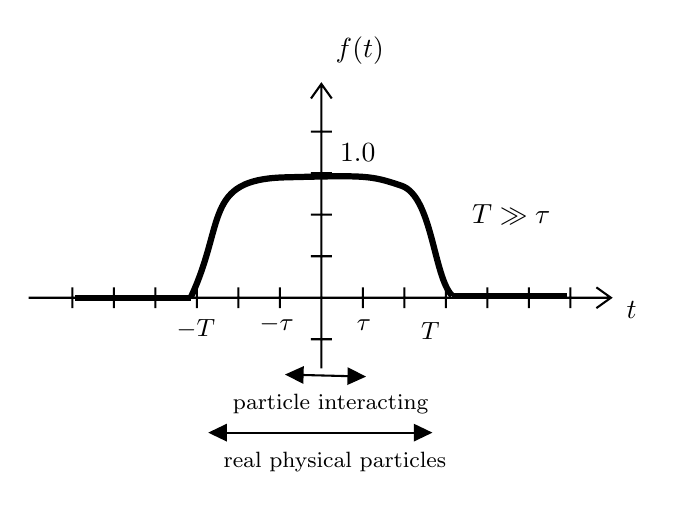
\begin{tikzpicture}[x=0.75pt,y=0.75pt,yscale=-1,xscale=1]
%uncomment if require: \path (0,300); %set diagram left start at 0, and has height of 300

%Shape: Axis 2D [id:dp9053022602492881] 
\draw [line width=0.75]  (206.5,193) -- (487,193)(347.5,90) -- (347.5,227) (480,188) -- (487,193) -- (480,198) (342.5,97) -- (347.5,90) -- (352.5,97) (367.5,188) -- (367.5,198)(387.5,188) -- (387.5,198)(407.5,188) -- (407.5,198)(427.5,188) -- (427.5,198)(447.5,188) -- (447.5,198)(467.5,188) -- (467.5,198)(327.5,188) -- (327.5,198)(307.5,188) -- (307.5,198)(287.5,188) -- (287.5,198)(267.5,188) -- (267.5,198)(247.5,188) -- (247.5,198)(227.5,188) -- (227.5,198)(342.5,173) -- (352.5,173)(342.5,153) -- (352.5,153)(342.5,133) -- (352.5,133)(342.5,113) -- (352.5,113)(342.5,213) -- (352.5,213) ;
\draw   ;
%Curve Lines [id:da8886982227128627] 
\draw [line width=2.25]    (284.5,193) .. controls (301.5,157) and (290.5,136) .. (330,135) .. controls (369.5,134) and (371,134) .. (386,139) .. controls (401,144) and (401.5,183) .. (410.5,192) ;
%Straight Lines [id:da30631719179412054] 
\draw [line width=2.25]    (229,193) -- (284.5,193) ;
%Straight Lines [id:da37700147882960855] 
\draw [line width=2.25]    (410.5,192) -- (466,192) ;
%Straight Lines [id:da753932751515977] 
\draw    (333,230.08) -- (366,230.92) ;
\draw [shift={(369,231)}, rotate = 181.47] [fill={rgb, 255:red, 0; green, 0; blue, 0 }  ][line width=0.08]  [draw opacity=0] (8.93,-4.29) -- (0,0) -- (8.93,4.29) -- cycle    ;
\draw [shift={(330,230)}, rotate = 1.47] [fill={rgb, 255:red, 0; green, 0; blue, 0 }  ][line width=0.08]  [draw opacity=0] (8.93,-4.29) -- (0,0) -- (8.93,4.29) -- cycle    ;
%Straight Lines [id:da09199346946537101] 
\draw    (296,258) -- (398,258) ;
\draw [shift={(401,258)}, rotate = 180] [fill={rgb, 255:red, 0; green, 0; blue, 0 }  ][line width=0.08]  [draw opacity=0] (8.93,-4.29) -- (0,0) -- (8.93,4.29) -- cycle    ;
\draw [shift={(293,258)}, rotate = 0] [fill={rgb, 255:red, 0; green, 0; blue, 0 }  ][line width=0.08]  [draw opacity=0] (8.93,-4.29) -- (0,0) -- (8.93,4.29) -- cycle    ;

% Text Node
\draw (365,123) node   [align=left] {1.0};
% Text Node
\draw (366,74) node    {$f( t)$};
% Text Node
\draw (497,199) node    {$t$};
% Text Node
\draw (287,208) node  [font=\small]  {$-T$};
% Text Node
\draw (400,209) node  [font=\small]  {$T$};
% Text Node
\draw (326,206) node  [font=\small]  {$-\tau $};
% Text Node
\draw (368,206) node  [font=\small]  {$\tau $};
% Text Node
\draw (439,153) node    {$T\gg \tau $};
% Text Node
\draw (352,244) node  [font=\footnotesize] [align=left] {particle interacting};
% Text Node
\draw (354,272) node  [font=\footnotesize] [align=left] {real physical particles};


\end{tikzpicture}

    \caption{The adiabatic hypothesis}
    \label{fig:adiabatic-hypothesis}
\end{figure}
Prior to $-T$, the particles are bare (ie, as $|i\rangle$). After $-T$, they become "dressed" due to self interaction, but are not close enough yet to interact with one another. At $t=-\tau$, they become close chough to interact with one another, which continues until $\tau$. The dressed particles then move apart and cease interacting, but remain dressed until $T$. At $T$, self-interaction ceases leaving the outgoing particles as bare, once again (i.e., as $|f\rangle$ ).

This is all fiction, of course, due in part to the fact that bare particle are never seen in the physical world and can never be measured. \bluep{But it allows us to use our math expressions which take $|i\rangle$ and $|f\rangle$ to be bare particles. After all our calculations are done, we take $T\to\infty$ to restore our fiction to reality.}

\section{Chapter Summary}
\subsection{The Renormalization Procedure}
1. Draw all relevant Feynman diagrams with 2 to $2 n$ vertices.

2. Add all the related Feynman amplitudes.

3. Evaluate all the propagator integrals in the amplitudes via regularization, yielding quantities $e$ and $m$ dependent on $\mathrm{e}_0$ and $\mathrm{m}_0$ respectively, and a parameter $\Lambda,$ wherein $e$ and $m$ become infinite when $\Lambda \rightarrow \infty$. Other quantities will be obtained that are finite and not dependent on $\Lambda$. These other quantities modify propagators and vertex relations.

4. Redefine $e_0$ and $m_0$ such that, as $\Lambda \rightarrow \infty, e$ and $m$ equal the finite, physical values for the QED charge constant and fermion particle (rest) mass. $e$ is dependent on interaction energy level $p$ and is expressed as $e(p)$.

\subsection{Solving Scattering Problems to Order n}
1. Write down the tree level amplitude with bare quantities $e_{0}$ and $m_{0}$

2. Replace $e_0$ and $m_0$ with renormalized values $e(p)$ and $m$, where $p$ is the energy level of the interaction, $m$ is the measured particle (rest) mass, and $e(p)$ is measured charge at energy level $p$.

3. Replace propagators with modified propagators

4. Replace the vertex relations with modified vertex relations.

\section{Solved Exercises}
1. Does it make sense to you that for our mass renormalization, we can have limit $\lim_{\Lambda\to\infty}\delta m=(\text { constant }) \lim_{\Lambda\to\infty} e_{0}^{2} \ln \frac{\Lambda}{m}=\infty$ and $e_{0}^{2}=0,$ whereas in our charge renormalization, we have (different constant) $\lim_{\Lambda\to\infty}e_{0}^{4} \ln \frac{k}{\Lambda}=e^{2}(k)$ = finite and $e_{0}^{2}=0$ ? Why?

\textbf{Solution:}

Note first that $\ln \frac{1}{\Lambda}=-\ln \Lambda$ and the minus sign can be part of a constant. So, consider, as $\Lambda\to\infty$, $e^2_0ln\Lambda=\infty$ and $e^4_0ln\Lambda=finite$. It makes sense because $e^4_0ln\Lambda=finite$ means $e_{0}^{4} \propto \frac{1}{\ln \Lambda}$. So, $e_{0}^{2} \propto \frac{1}{\sqrt{\ln \Lambda}}, e_{0}^{4} \ln \Lambda \propto \frac{1}{\ln \Lambda} \ln \Lambda=1$, but $e_{0}^{2} \ln \Lambda \propto \frac{1}{\sqrt{\ln \Lambda}} \ln \Lambda=\sqrt{\ln \Lambda}$ goes $\to\infty$ as $\Lambda\to\infty$. For $\Lambda\to\infty$,$e_{0}^{2} \propto \frac{1}{\sqrt{\ln \Lambda}} \rightarrow 0 , e_{0}^{4} \propto \frac{1}{\ln \Lambda} \rightarrow 0$.

2. Determine what the QED coupling constant will be at $6.0 \mathrm{MeV}$. (You need to assume the evaluation is at a virtually immeasurable amount less than $6.0 \mathrm{MeV}$.) Then determine what the coupling constant is at $12.0 \mathrm{MeV}$ (i.e., immeasurably below 12.0 ).

$$
\alpha(6.0) \approx\frac{1}{137}\left(1+\frac{1}{137} 8 \pi\frac{1}{12 \pi^{2}} \ln \frac{6.0}{1.022}\right)=\frac{1}{137}\left(1+\frac{1}{137} \frac{2}{3 \pi}(1.770)\right)\approx \frac{1}{136.63}
$$

Now use the above value as the starting point for the next calculation. Up/anti-up loops contribute from $6.0$ MeV upward, but down/anti-down loops don't contribute below 12 MeV. So now $\mu=6.0$ MeV and $p=12.0$ MeV, with 
$$b_{n}=\frac{1}{12 \pi^{2}}\left((1)^{2}+1 \cdot 3\left(\frac{2}{3}\right)^{2}+0\right)=\frac{1}{12 \pi^{2}}\left(\frac{3}{3}+\frac{4}{3}\right)=\frac{7}{36 \pi^{2}}$$

$$\alpha(p) \approx \alpha(\mu)\left(1+\alpha(\mu) 8 \pi b_{n} \ln \frac{p}{\mu}\right)=\frac{1}{136.28}$$